\chapter[Related Works]{Related works}
\section[Volatility]{Volatility}

Volatility \cite{volatility} is an open-source forensics tool first developed
by Aaron. The four developers of this project also publish the book on memory
forensics, The Art of Memory Forensics.

Volatility is written in Python 2, and the project is being rewritten (2020) in
Python 3. The project is a result of many research in memory forensics in
Windows, Linux, and MacOS. Volatility only works on memory file, and support
many memory file formats.

To find malware in Windows, Volatility has commands to list processes, kernel
modules, inspect the SSDT and IRP, and list unloaded drivers. Volatility also
employs pool tag scanning to find processes, threads, drivers, kernel modules,
network connections, kernel callbacks. Volatility has a command to compare the
process lists produced by traversing different process list and pool tag
scanning for processes, \texttt{psxview}.  Figure \ref{fig:volatility} shows
the sample output of the Volatility's \texttt{psxview} commands.

\begin{figure}[h]
  \centering
  \caption{Volatility}
  \label{fig:volatility}
  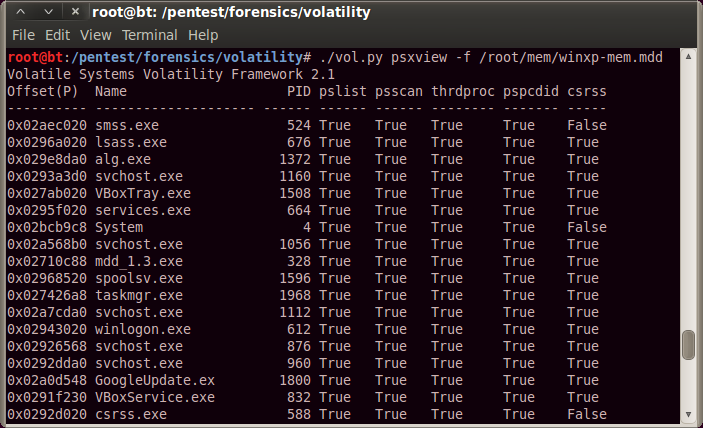
\includegraphics[scale=0.5]{images/volatility.png}
\end{figure}

Volatility is a versatile and powerful tool ever created to tackle the memory
forensics. It can work on memory dumps of different Windows versions and help
investigators explore many data related to the system.

\section[Rekall]{Rekall}

Rekall open-source project by Google \cite{rekall} is the second choice in
memory forensics.  Rekall is also written in Python 2 and provides almost the
same functionalities that Volatility has. Rekall uses the debug symbols to
resolve the structures layout and global variable offsets in Windows analysis.
One withdrawal from Rekall is probably the installation, where Rekall is harder
to install and use than Volatility.

Rekall has a memory capture module called WinPmem, which is also a kernel
driver for doing live forensics. On doing live memory forensics, WinPmem
creates a device at \texttt{\textbackslash\textbackslash .\textbackslash pmem}
and Rekall will perform the forensics on the device.

Rekall performs live forensics by mapping every physical memory pages and binds
the read operation to \texttt{\textbackslash\textbackslash .\textbackslash
pmem} in \texttt{IRP\_MJ\_READ}. When the user application read the file at an
offset, WinPmem driver will map the required physical page and copy to the
output buffer.

\section[Memtriage]{Memtriage}

Memtriage \cite{memtriage} is a wrapper around the Rekall WinPmem driver and
Volatility to do live forensics with Volatility.  This project can make
Volatility works on live systems with limitations. There have been crashes
reported on some Windows versions.


\section[SysInternal]{SysInternal}

Sysinternals \cite{sysinternal} is a suite of programs made by Mark
Russinovich, now redistributed by Windows. Two programs that are used by
malware analysts to inspect the system are Process Explorer and Process
Monitor.  Process Explorer is a Task manager with verbose information. Process
Explorer uses Windows API to query the systems for process and threads
information.  Process Monitor captures events by Windows and displays them in a
GUI. Process Monitor can capture process/thread creation, termination, file
access, registry access, network activities and many more. On a live machine,
Process Monitor is handy to know what process is doing so that malware analysts
can narrow down process by process to find the malware writing registry values,
edit a file, or connecting to a remote server.


\begin{figure}[h]
  \centering
  \caption{Process Explorer}
  \label{fig:processexp}
  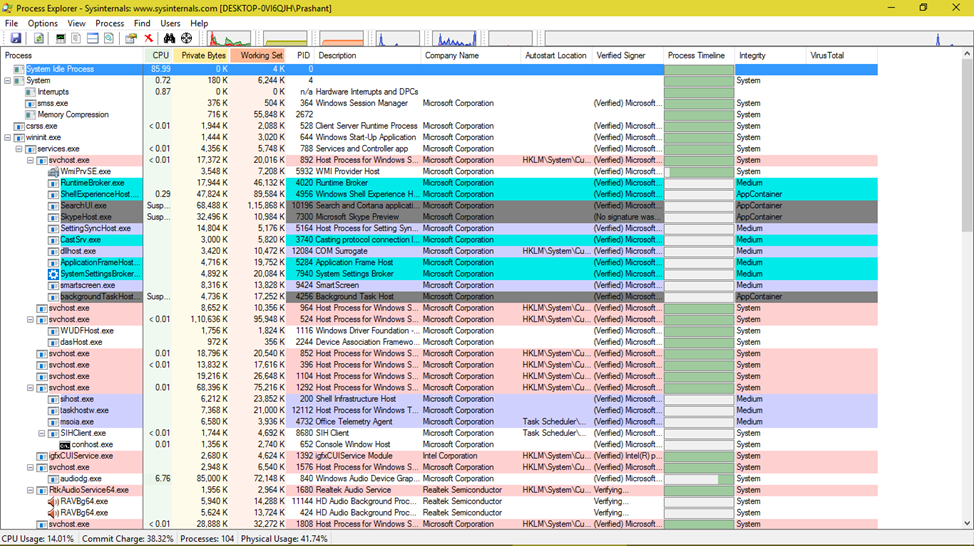
\includegraphics[scale=0.4]{images/processexp.png}
\end{figure}

\begin{figure}[h]
  \centering
  \caption{Process Monitor}
  \label{fig:processmon}
  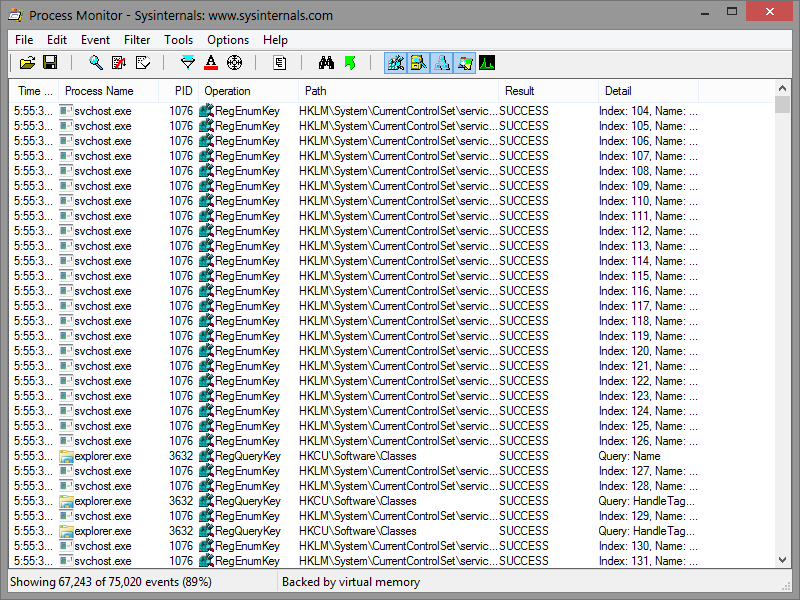
\includegraphics[scale=0.5]{images/processmon.png}
\end{figure}

\section[Process hacker]{Process hacker}

The Process Hacker \cite{processhacker} is an open-source project maintained by
Wen Jia Liu and Steven G. The goal of this project is to give the user a tool
to monitor system resources, debug software, and detect malware. Process Hacker
has a graphical user interface to inspect processes, network connections, file
access. Process Hacker also uses a kernel driver to capture stack traces,
enumerating process handler more efficiently, retrieving names for file
handlers and EtwRegistration objects, and setting handle attributes.

Process hacker does not use any forensics methods to detect malware, but either
using more verbose information into the system to let the user know what
processes are doing.


\begin{figure}[h]
  \centering
  \caption{Process Hacker}
  \label{fig:processhacker}
  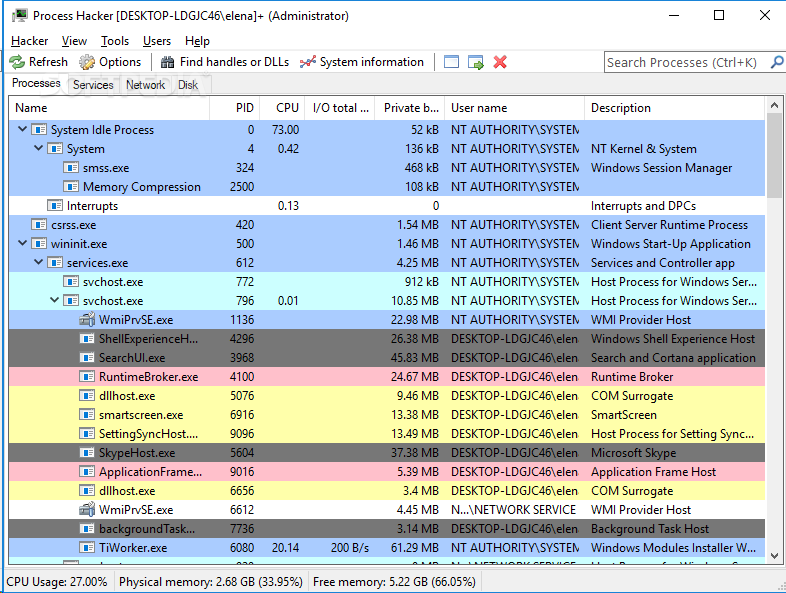
\includegraphics[scale=0.7]{images/processhacker.png}
\end{figure}


